\section{Bosim. Paskal qonuni}

\begin{enumerate}

\item Atmosfera tomga 20 MN kuch bilan ta’sir qilmoqda. Atmosfera bosimi 100 kPa 
bo‘lsa, tomning yuzasini toping (m$^2$). 

\begin{enumerate}[label=\Alph*)]
\item 20
\item 50
\item 200
\item 30
\end{enumerate}



\item Massasi 4 kg va yuzi 8 m$^2$ bo‘lgan gilam polga qanday bosim beradi (Pa)? 

\begin{enumerate}[label=\Alph*)]
\item 0,2
\item 0,5
\item 2
\item 5
\end{enumerate}

\item Nasos gidravlik pressga moyni 300 N/cm$^2$ bosim bilan yuboradi. 
Katta porshenning kesim yuzi 900 cm$^2$ bo‘lsa, u qanday kuch bilan ta’sir etadi (kN)? 
\begin{enumerate}[label=\Alph*)]
\item 250
\item 90
\item 270
\item 300

\end{enumerate}

\item Rasmda uchta g‘isht stol ustiga to‘rt holatda qo‘yilgan. Qaysi holatda g‘ishtlar stolni kattaroq kuch bilan bosadi? 

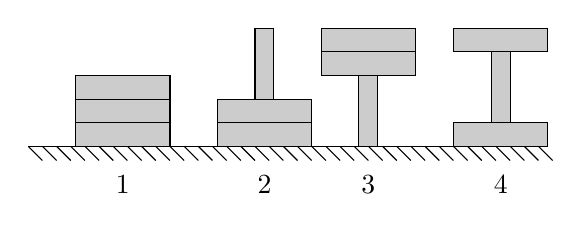
\begin{tikzpicture}[scale=0.6]

% yer (shtrix)
\draw (-1,0) -- (10,0);
\foreach \x in {-1,-0.7,...,10}
{
\draw (\x,0) -- (\x+0.3,-0.3);
}

% --- 1-holat ---
\draw[fill=gray!40] (0,0) rectangle (2,0.5);
\draw[fill=gray!40] (0,0.5) rectangle (2,1);
\draw[fill=gray!40] (0,1) rectangle (2,1.5);
\node at (1,-0.8) {1};

% --- 2-holat ---
\draw[fill=gray!40] (3,0) rectangle (5,0.5);
\draw[fill=gray!40] (3,0.5) rectangle (5,1);
\draw[fill=gray!40] (3.8,1) rectangle (4.2,2.5);
\node at (4,-0.8) {2};

% --- 3-holat ---
\draw[fill=gray!40] (6,0) rectangle (6.4,2);
\draw[fill=gray!40] (5.2,1.5) rectangle (7.2,2);
\draw[fill=gray!40] (5.2,2) rectangle (7.2,2.5);
\node at (6.2,-0.8) {3};

% --- 4-holat ---
\draw[fill=gray!40] (8,0) rectangle (10,0.5);
\draw[fill=gray!40] (8.8,0.5) rectangle (9.2,2);
\draw[fill=gray!40] (8,2) rectangle (10,2.5);
\node at (9,-0.8) {4};

\end{tikzpicture}
\begin{enumerate}[label=\Alph*)]
\item 1
\item 2
\item 3

\item hamma holatlarda bir xil kuch bilan bosadi.
\end{enumerate}



\item G‘isht stol ustiga rasmda tasvirlangandek 3 xil holatda qo‘yilgan. G‘ishtning qaysi holatida uning stolga bosimi eng katta? 

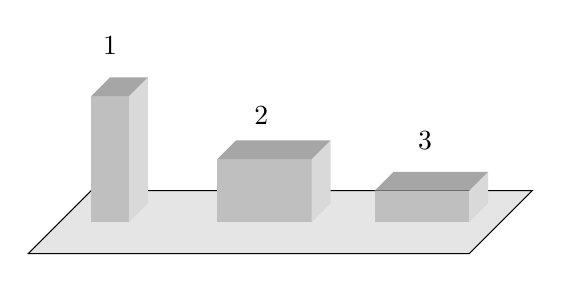
\begin{tikzpicture}[scale=0.8]

% --- platforma (stol) ---

\fill[gray!20] (0,0.2) -- (7,0.2) -- (8,1.2) -- (1,1.2) -- cycle;
\draw (0,0.2) -- (7,0.2) -- (8,1.2) -- (1,1.2) -- cycle;

% --- 1-holat (tik) ---
\fill[gray!50] (1,0.7) rectangle (1.6,2.7);
\fill[gray!30] (1.6,0.7) -- (1.9,1) -- (1.9,3) -- (1.6,2.7) -- cycle;
\fill[gray!70] (1,2.7) -- (1.6,2.7) -- (1.9,3) -- (1.3,3) -- cycle;
\node at (1.3,3.5) {1};

% --- 2-holat (yonboshlab) ---
\fill[gray!50] (3,0.7) rectangle (4.5,1.7);
\fill[gray!30] (4.5,0.7) -- (4.8,1) -- (4.8,2) -- (4.5,1.7) -- cycle;
\fill[gray!70] (3,1.7) -- (4.5,1.7) -- (4.8,2) -- (3.3,2) -- cycle;
\node at (3.7,2.4) {2};

% --- 3-holat (yotgan) ---
\fill[gray!50] (5.5,0.7) rectangle (7,1.2);
\fill[gray!30] (7,0.7) -- (7.3,1) -- (7.3,1.5) -- (7,1.2) -- cycle;
\fill[gray!70] (5.5,1.2) -- (7,1.2) -- (7.3,1.5) -- (5.8,1.5) -- cycle;
\node at (6.3,2) {3};

\end{tikzpicture}

\begin{enumerate}[label=\Alph*)]
\item 1
\item 2
\item 3
\item hamma holatlarda bosim bir xil.

\end{enumerate}

\item Diametri 2 marta ortganda, doira shaklidagi sirtga biror kuchning bosimi qanday 
o‘zgaradi? 
\begin{enumerate}[label=\Alph*)]
\item 2 marta ortadi.
\item 2 marta kamayadi. 
\item 4 marta ortadi.
\item 4 marta kamayadi.
\end{enumerate}

\item Bino bir nechta granit ustunlarga ega bo‘lib, har bir ustunning hajmi 9 m$^3$ ga, asosining yuzi 1,4 m$^2$ ga teng. Granitning zichligi 2800 kg/m$^3$. Bitta ustun o‘z og‘irligi ta’sirida poydevorga qancha bosim (kPa) beradi? 
\begin{enumerate}[label=\Alph*)]
\item 160
\item 200
\item 180
\item 220
\end{enumerate}

\item Blokka osilgan jismlar rasmdagi kabi muvozanatda turibdi. Katta yukning stol sirtiga tegib turgan qismining yuzi 0,4 m$^2$ bo‘lsa, u stolga necha Pa bosim bermoqda? 

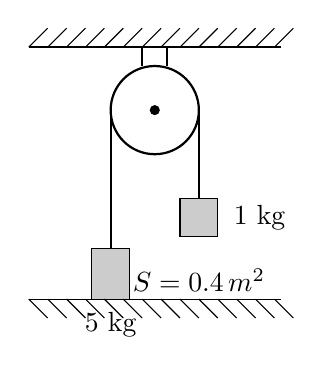
\begin{tikzpicture}[scale=0.8]

% --- shift (tepa) ---
\draw[thick] (-2,4) -- (2,4);
\foreach \x in {-2,-1.7,...,2}
{
\draw (\x,4) -- (\x+0.3,4.3);
}

% --- blok (g‘ildirak) ---
\draw[thick] (0,3) circle (0.7);
\fill (0,3) circle (0.08);

% tayanch
\draw[thick] (-0.2,4) -- (-0.2,3.7);
\draw[thick] (0.2,4) -- (0.2,3.7);

% --- ip ---
\draw[thick] (-0.7,3) -- (-0.7,0.8);
\draw[thick] (0.7,3) -- (0.7,1.6);

% --- chap yuk (5 kg) ---
\draw[fill=gray!40] (-1,0) rectangle (-0.4,0.8);
\node at (-0.7,-0.4) {5 kg};

% stol
\draw (-2,0) -- (2,0);
\foreach \x in {-2,-1.7,...,2}
{
\draw (\x,0) -- (\x+0.3,-0.3);
}

% S yozuvi
\node at (0.7,0.3) {$S=0.4\,\text{m}^2$};

% ipdan yukga
\draw[thick] (-0.7,1) -- (-0.7,1);

% --- o‘ng yuk (1 kg) ---
\draw[fill=gray!40] (0.4,1) rectangle (1,1.6);
\node[right] at (1.1,1.3) {1 kg};

\draw[thick] (0.7,1.2) -- (0.7,1.2);

\end{tikzpicture}
\begin{enumerate}[label=\Alph*)]
\item 100
\item 400
\item 200
\item 500
\end{enumerate}

\item $F=120$ N kuch $S=0,6$ m$^2$ yuzaga vertikalga nisbatan $\alpha=37^\circ$ burchak ostida ta’sir qilmoqda. Bu kuchning bosimini aniqlang (Pa). 

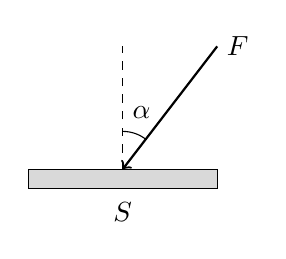
\begin{tikzpicture}[scale=0.6]

% --- sirt (S) ---
\draw[fill=gray!30] (-2,0) rectangle (2,0.4);
\node at (0,-0.5) {$S$};

% --- vertikal (punktir) ---
\draw[dashed] (0,0.4) -- (0,3);

% --- kuch F ---
\draw[<-,thick] (0,0.4) -- (2,3);
\node[right] at (2,3) {$F$};

% --- burchak alpha ---
\draw (0,1.2) arc (90:52:0.8);
\node at (0.4,1.6) {$\alpha$};

\end{tikzpicture}

\begin{enumerate}[label=\Alph*)]
\item 120
\item 300
\item 240
\item 160
\end{enumerate}

\item Qirrasining uzunligi 2 m bo‘lgan kub shaklidagi og`irligi 20 N bo`lib u qiya tekislik ustida tinch turibdi. Jismning qiya tekislik yuzasiga berayotgan bosimini aniqlang (Pa). 

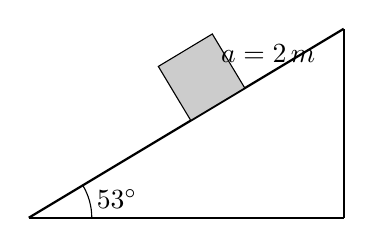
\begin{tikzpicture}[scale=0.8]

% --- qiya tekislik ---
\draw[thick] (0,0) -- (5,0);        % asos
\draw[thick] (0,0) -- (5,3);        % qiya tomon
\draw[thick] (5,0) -- (5,3);        % tik tomon

% --- blok ---
\begin{scope}[rotate=31] % ~53° ga mos vizual
\draw[fill=gray!40] (3,0) rectangle (4,1);
\end{scope}

% --- burchak (53°) ---
\draw (1,0) arc (-180:-149:-1);
\node at (1.4,0.3) {$53^\circ$};

% --- uzunlik yozuvi ---
\node at (3.8,2.6) {$a=2\,\text{m}$};

\end{tikzpicture}

\begin{enumerate}[label=\Alph*)]
\item 5
\item 4
\item 3
\item 2
\end{enumerate}

\item Paskal qonunining to‘g‘ri ta’rifini ko‘rsating. 
\begin{enumerate}[label=\Alph*)]
\item Suyuqlik yoki gazlarga ko‘rsatilgan tashqi bosim ularning hamma nuqtalariga o‘zgarishsiz uzatiladi. 
\item Muvozanatdagi barcha jismlarga berilgan tashqi bosim hamma tomonga bir xil uzatiladi.
\item Suyuqlikka botirilgan jism o‘z og‘irligini qisman yo‘qotadi. 
\item Atmosfera og‘irligi tufayli yerga bosim bilan ta’sir etadi. 

\end{enumerate}

\item Berk idishdagi suyuqliklar va gazlar o‘zlariga berilgan tashqi bosimni ... 
\begin{enumerate}[label=\Alph*)]
\item shu bosim yo‘nalishi bo‘yicha uzatadi. 
\item hamma yo‘nalishlarda bir xil uzatadi. 
\item shu bosimga tik yo‘nalish bo‘yicha uzatadi. 
\item ta’sir etuvchi kuchga qarama-qarshi yo‘nalishda uzatadi. 
\end{enumerate}


\item ... ko‘rsatilgan tashqi bosim barcha yo‘nalishlarda bir xil uzatiladi. 
\begin{enumerate}[label=\Alph*)]
\item faqat suyuqliklarda.
\item faqat gazlarda. 
\item gazlar va suyuqliklarda.
\item qattiq jismlarda. 
\end{enumerate}

\item Ichiga havo qamalgan koptokni siqsak, bosim qayerda ko‘proq ortadi? 
\begin{enumerate}[label=\Alph*)]
\item kuch yo‘nalishida.
\item barcha nuqtasida.
\item pastki qismida.
\item yuqori qismida.

\end{enumerate}
\end{enumerate}





\begin{table}[h!]
\centering
\begin{tabular}{|c|c|c|c|c|c|c|}
\hline
№ & J. & № & J. & № & J.  \\ \hline
1 & C & 6 & D & 11 & A \\ \hline
2 & D & 7 & C & 12 & B \\ \hline
3 & C & 8 & A & 13 & C \\ \hline
4 & C & 9 & D & 14 & B  \\ \hline
5 & A & 10 & A & 15 &   \\ \hline
\end{tabular}
\end{table}